\documentclass{article}[12pt]

\usepackage[utf8]{inputenc}
\usepackage{amsfonts,amssymb,amsmath,subfigure}
\usepackage[pdftex]{graphicx}
\usepackage{epstopdf}
\usepackage{vmargin}
\usepackage{comment}
\usepackage{tikz,multicol}

\usepackage{algorithm}
\usepackage[noend]{algpseudocode}
\usepackage{tcolorbox}
\usepackage{cancel}


\newcommand*{\esp}{\mathbb{E}} 
\newcommand*{\prob}{\mathsf{P}}
\newcommand*{\var}{\mathbb{V}}
\newcommand*{\cov}{\mathbb{C}\mathsf{ov}}
\newcommand*{\Si}{\textbf{Si }}
\newcommand*{\finsi}{\textbf{Fin si }}
\newcommand*{\alors}{\textbf{alors }}
\newcommand*{\tantque}{\textbf{Tant que }}
\newcommand*{\fintantque}{\textbf{Fin tant que }}
\newcommand*{\pour}{\textbf{Pour }}
\newcommand*{\finpour}{\textbf{Fin pour }}
\newcommand*{\allant}{\textbf{ allant de }}
\newcommand*{\jusqua}{\textbf{ à }}
\newcommand*{\res}{\textbf{Retourner }}


\newtcolorbox{mybox}[3][]
{
  colframe = #2!25,
  colback  = #2!10,
  coltitle = #2!20!black,  
  title    = {#3},
  #1,
}


\newcommand*\Let[2]{\State #1 $\gets$ #2}
\algrenewcommand\algorithmicrequire{\textbf{Precondition:}}
\algrenewcommand\algorithmicensure{\textbf{Postcondition:}}




\excludecomment{solution}
%\includecomment{solution}

\title{IF111 - Algorithmes et structures de données\\E2 - Récursivité et Diviser pour régner}
\date{\texttt{rfosse@labri.fr}}
\author{Rohan Fossé}
\begin{document}



\maketitle{}

\section{Récursivité}

\subsection*{Exercice 1}
\begin{enumerate}
\item Flemme



        \item Soit $D(k)$ le nombre de déplacement à l'étage $k$
        \begin{align*}
            D(k) &= 2D(k-1)\\
            D(1) &= 1\\
            \Rightarrow D(k) &= 2^{k-1}
        \end{align*}
        
        Il y a $n$ étages pour $n$ disques à déplacer et pour l'étage $k
        $, on dénombre $2^{k-1}$ déplacement. Le nombre $T_D(n)$ de déplacement total est :
        
        \begin{align*}
            T_D(n) &= \sum_{k=1}^{n}2^{k-1}\\
            & = \frac{1-2^n}{1-2}
        \end{align*}
        \begin{center}
            \begin{tcolorbox}[text width = 2.8cm]
                $T_D(n) = 2^n -1$
            \end{tcolorbox}
        \end{center}
\end{enumerate}

\subsection*{Exercice 2}
    On a $F(5) = 5$
    \begin{figure}[h!]
            \centering
            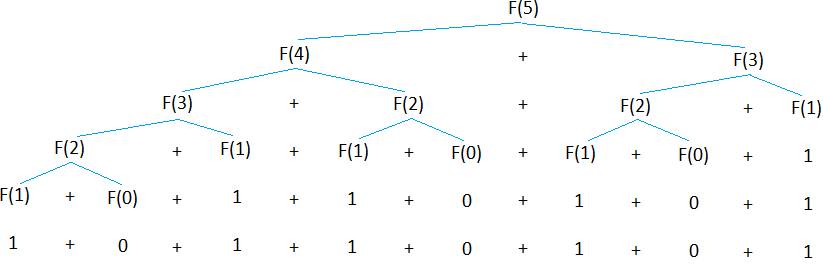
\includegraphics[scale = 0.91]{Fibonacci.png}
    \end{figure}



\begin{algorithm}
\caption{Calcul du nième terme de la suite de Fibonacci}
\begin{algorithmic}[1]
\State\textbf{Fib}(n)
\State \qquad CréerTableauEntier(n) \textit{T}
\State \qquad $\textit{T}[0] \gets 0$
\State \qquad $\textit{T}[1] \gets 1$

\State \qquad \pour \textit{i} \allant2\jusqua \textit{n}
\State \qquad \qquad $\textit{T}[i] \gets \textit{T}[i-2] + \textit{T}[i-1]$
\State \qquad \finpour
\State \qquad \res$\textit{T}[n]$
\end{algorithmic}
\end{algorithm}

Toutes les additions ont lieu dans la boucle $\pour$et on en compte une pour chaque itération. \begin{center}
    \begin{tcolorbox}[text width = 7cm]
        Ce qui fait un total de $n-1$ additions.
    \end{tcolorbox}
\end{center}

\underline{remarque :}
\begin{align*}
    F(n) - F(n-1) - F(n-2) = 0 \Rightarrow &X^2 - X - 1 = 0\\
    & X = \frac{1 \pm \sqrt{5}}{2}
\end{align*}
\begin{align*}
    F(n) &= \alpha \left(\frac{1 + \sqrt{5}}{2}\right)^n + \beta \left(\frac{1 -1 \sqrt{5}}{2}\right)^n\\\\
    F(0) &= 0 \Leftrightarrow \alpha + \beta = 0\\
    F(1) &= 1 \Leftrightarrow \alpha \frac{1 + \sqrt{5}}{2} + \beta \frac{1 -1 \sqrt{5}}{2}\\
    &\Rightarrow \alpha = \frac{1}{\sqrt{5}} \text{ et } \beta = -\frac{1}{\sqrt{5}}
\end{align*}
\begin{center}
    \begin{tcolorbox}[text width = 9.5cm]
        \[F(n) = \frac{1}{\sqrt{5}}\left(\frac{1 + \sqrt{5}}{2}\right)^n - \frac{1}{\sqrt{5}}\left(\frac{1 - \sqrt{5}}{2}\right)^n\]
    \end{tcolorbox}
\end{center}

\subsection*{Exercice 3}

\begin{figure}[h!]
    \centering
        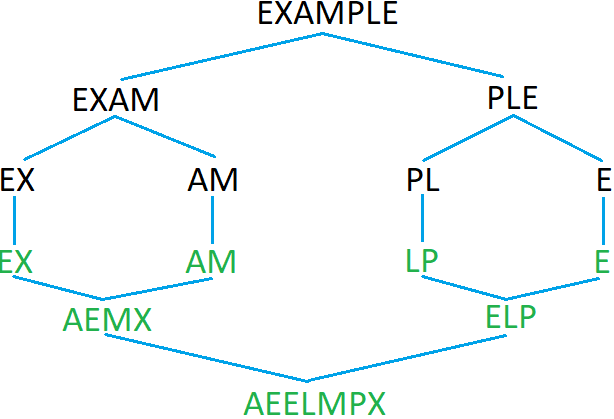
\includegraphics[scale = 1]{EXAMPLE.png}
\end{figure}

\newpage


\subsection*{Exercice 4}
\begin{solution} 
\paragraph{Solution} 
\begin{tabbing}
~~~~\=~~~~\=~~~~\=~~~~\=~~~~\=\kill
\> \textbf{IndexMax(T,i,j)}\\
1.\> \{ entier max;\\
2.\> \textbf{si} $(i=j)$ \textbf{alors} \textbf{retourner} $i$\\
3.\> \textbf{sinon} \\
4.\> \> $m \leftarrow ( \lfloor \frac{i+j}{2}\rfloor)$;\\
5. \> \> $max_1 \leftarrow IndexMax(T,i,m)$ ;\\
6. \> \> $max_2 \leftarrow IndexMax(T,m+1,j)$ ;\\
7. \> \> \textbf{si} $T[max_1]<T[max_2]$ \textbf{retourner} $max_2$\\
8. \> \> \textbf{sinon} \textbf{retourner} $max_1$\\
9. \> \> \textbf{fin si}\\
10. \> \textbf{fin si}\\
11.\> \}
\end{tabbing}

Récurrence : $T(n)= T(\lceil (\frac{n}{2}\rceil)+T(\lfloor\frac{n}{2}\rfloor)+1$ pour $n>1$, $T(1)$=0\\
On considère $n=2^k$, $T(n)=2T(\frac{n}{2})+1$=\\
=$2(2T(\frac{n}{4})+1)+1=4T(\frac{n}{4})+3$=\\
= $4 (2 T(\frac{n}{8})+1)+3=8 T(\frac{n}{8})+7$=\\
= $i T(\frac{n}{i})+i-1$. $\frac{n}{i}=1$ pour $n=i$\\
= $ n T(1)+n-1$= n-1
exo 4.1 Ananin Levityn 
\end{solution}

\begin{algorithm}
\caption{Le plus grand élément dans un tableau avec la méthode diviser-pour-régner}
\begin{algorithmic}[1]
\State\textbf{MaxRec}(\textit{T})
\State \qquad entier $n \gets \text{Taille de } \textit{T}$
\State \qquad \Si n = 1 \alors
\State \qquad \qquad \res$\textit{T}[1]$
\State \qquad \finsi
\State \qquad \res le maximum entre $\textbf{MaxRec}\left(\textit{T}1,\left\lfloor\dfrac{n}{2}\right\rfloor\right)$ et $\textbf{MaxRec}\left(\textit{T}\left\lfloor\dfrac{n}{2}\right\rfloor + 1, n\right)$
\end{algorithmic}
\end{algorithm}
Mais cet algorithme ne donne pas la position du maximum dans le tableau \textit{T}. Soit C le nombre de comparaison et $n = 2^p$ le nombre d'éléments dans le tableau.
\begin{align*}
    C(k) &= 2C\left(\frac{k}{2}\right)\\
    C(2^p) &= 2^p C(1)
\end{align*}
\begin{center}
    \begin{tcolorbox}[text width = 3.5cm]
        \[C(n) = 2^p\]
    \end{tcolorbox}
\end{center}


\begin{tabbing}
~~~~\=~~~~\=~~~~\=~~~~\=~~~~\=\kill
\> \textbf{IndexMax(T,i,j)}\\
1.\> \{ entier max;\\
2.\> \textbf{si} $(i=j)$ \textbf{alors} \textbf{retourner} $i$\\
3.\> \textbf{sinon} \\
4.\> \> $m \leftarrow ( \lfloor \frac{i+j}{2}\rfloor)$;\\
5. \> \> $max_1 \leftarrow IndexMax(T,i,m)$ ;\\
6. \> \> $max_2 \leftarrow IndexMax(T,m+1,j)$ ;\\
7. \> \> \textbf{si} $T[max_1]<T[max_2]$ \textbf{retourner} $max_2$\\
8. \> \> \textbf{sinon} \textbf{retourner} $max_1$\\
9. \> \> \textbf{fin si}\\
10. \> \textbf{fin si}\\
11.\> \}
\end{tabbing}

Récurrence : $T(n)= T(\lceil (\frac{n}{2}\rceil)+T(\lfloor\frac{n}{2}\rfloor)+1$ pour $n>1$, $T(1)$=0\\
On considère $n=2^k$, $T(n)=2T(\frac{n}{2})+1$=\\
=$2(2T(\frac{n}{4})+1)+1=4T(\frac{n}{4})+3$=\\
= $4 (2 T(\frac{n}{8})+1)+3=8 T(\frac{n}{8})+7$=\\
= $i T(\frac{n}{i})+i-1$. $\frac{n}{i}=1$ pour $n=i$\\
= $ n T(1)+n-1$= n-1
exo 4.1 Ananin Levityn 


\newpage
\subsection*{Exercice 5}
\begin{algorithm}
\caption{Teste si E possède un élément \textit{majoritaire} et le renvoie le cas échéant}
\begin{algorithmic}[1]
\State\textbf{PossèdeMajoritaire}(\textit{T})
\State \qquad entier $n \gets \text{Taille de } \textit{E}$
\State \qquad CréerTableau(n) \textit{Unique}
\State \qquad entier $distinct \gets 0$
\State
\State \qquad \pour $x\in$ \textit{E}
\State \qquad \qquad \Si $x\notin$ \textit{Unique}
\State \qquad \qquad \qquad $\textit{Unique}[distinct]\gets x$
\State \qquad \qquad \qquad $distinct \gets distinct + 1$
\State \qquad \qquad \finsi
\State \qquad \finpour
\State
\State \qquad \Si $distinct \geq \frac{n}{2}$
\State \qquad \qquad \res $(-, 0)$
\State \qquad \finsi
\State
\State \qquad entier $c_x \gets 0$ ; entier $c \gets 0$  \qquad/*compteurs*/
\State \qquad entier $position_x \gets 1$
\State
\State \qquad \pour \textit{i}\allant1\jusqua \textit{distinct}
\State \qquad \qquad \pour $\textit{élément}\in \textit{E}$
\State \qquad \qquad \qquad \Si $\textit{Unique}[i] = \textit{élément}$
\State \qquad \qquad \qquad \qquad $c\gets c + 1$
\State \qquad \qquad \qquad \finsi
\State \qquad \qquad \finpour
\State \qquad \qquad \Si $c>c_x$
\State \qquad \qquad \qquad $c_x \gets c$
\State \qquad \qquad \qquad $position_x \gets i$
\State \qquad \qquad \finsi
\State \qquad \finpour
\State
\State \qquad \Si $c_x \leq \frac{n}{2}$
\State \qquad \qquad \res (-, 0)
\State \qquad \finsi
\State \qquad \res ($\textit{Unique}[position_x],\text{ }c_x$)
\end{algorithmic}
\end{algorithm}
Dans le pire des cas : $distinct = \frac{n}{2} - 1$\\
On fait alors $n$ comparaisons puis $distinct\times(n+1)$\\
Notons $T_{pire}(n)$ le total :
\begin{align*}
    T_{pire}(n) &= n + \left(\frac{n}{2} - 1\right)(n+1)\\
    &= \cancel{n} + \frac{n^2}{2} + \frac{n}{2} - \cancel{n} - 1
\end{align*}
\begin{center}
    \begin{tcolorbox}[text width = 5.7cm]
        \[T_{pire}(n) = \frac{n^2}{2} + \frac{n}{2} - 1\]
    \end{tcolorbox}
\end{center}

\newpage
\subsection*{Exercice 6}



\begin{tabbing}
~~~~\=~~~~\=~~~~\=~~~~\=~~~~\=\kill
\> \textbf{Compte0(T,i,j)}\\
1.\> \{\\
2.\> \textbf{si} $(i=j)$ ou $(i=j-1)$ \textbf{faire}\\
3.\> \> \textbf{tant que} $(T[i]\neq 1)$ et $(i\leq j)$ \textbf{faire}\\
4.\> \>\> $i\leftarrow i+1$;\\
5.\> \> $\textbf{fin tant que}$;\\
6.\> \> \textbf{retourner} $i-1$;\\
7.\> \textbf{sinon} \\
8.\> \> $m \leftarrow \lfloor (\frac{i+j}{2}) \rfloor$;\\
9. \> \> \textbf{si} $T[m]=1$ \textbf{alors} Compte0(T,i,m-1);\\
10. \> \> \textbf{sinon} Compte0(T,m+1,j);\\
11. \> \> \textbf{fin si}\\
12. \> \textbf{fin si}\\
13.\> \}
\end{tabbing}

\subsection*{Exercice 7}
\begin{enumerate}
    \item $b=2$, $a=4$, $d=1$ $d<log_2(4)$ $T(n)=O(n^2)$ cas 3 du théorème
    \item $T(n)=4T(n/2)+n^2$
    \item $b=2$, $a=4$, $d=2$ $d=log_2(4)$ $T(n)=O(n^2logn)$ cas 2 du théorème
\end{enumerate}


\section{Diviser pour régner}



\end{document} 